\medskip

\textbf{Partie A}

	\medskip

\begin{enumerate}
\item Dérivons la fonction $u$ :
\quad
$\begin{aligned}[t]
\forall t \in \R,\quad u'(t) &= 1 \times \e^{-0,4t} + t \times (-0,4)\e^{-0,4t} \\
&= \e^{-0,4t} - 0,4t\e^{-0,4t} \\
&= (1 - 0,4t)\e^{-0,4t}
\end{aligned}$

Vérifions que $u$ est solution de $(E)$ :

$\begin{aligned}[t] \forall t \in \R, \quad
u'(t) + 0,4u(t) &= (1 - 0,4t)\e^{-0,4t} + 0,4 \times t\e^{-0,4t}\\
&= \e^{-0,4t} - 0,4t\e^{-0,4t} + 0,4t\e^{-0,4t}\\
&= \e^{-0,4t}
\end{aligned}$

Donc $u$ est bien solution de $(E)$.

\item
	\begin{enumerate}
		\item Soit $g = f - u$ avec $g$ solution de $(H)$.

Comme $g$ est une solution de $(H)$, on a :\quad $\forall t \in \R, \quad g'(t) + 0,4g(t) = 0$.

Or $g = f - u$, donc $g' = f' - u'$.

Ainsi :

$\begin{aligned}[t]
\forall t \in \R, \quad g'(t) +0,4g(t) = 0
	&\iff f'(t) - u'(t) + 0,4\big(f(t) - u(t)\big) = 0 \\
	&\iff f'(t) - u'(t) + 0,4f(t) - 0,4u(t) = 0\\
	&\iff f'(t) + 0,4f(t) = u'(t)  + 0,4u(t)\\
	&\iff f'(t) + 0,4f(t) = \e^{-0,4t}\\
\end{aligned}$

La dernière équivalence se justifie car $u$ étant une solution particulière de $(E)$, on a bien:
\quad $\forall t \in \R, \quad u'(t) + 0,4u(t) = \e^{-0,4t}$, \quad où $C \in \R$.

Donc $f$ est solution de $(E)$.

\item L'équation $(H)$ : $y' + 0,4y = 0$ est de la forme $y' = - 0,4y$.

Les solutions sont les fonctions de la forme : $g : t \longmapsto C\e^{-0,4t}$ où $C \in \R$.

\item D'après les questions précédentes, $f$ est solution de $(E)$ si et seulement si \linebreak $g = f - u$ est solution de $(H)$.

	Donc si et seulement si on a :\quad  $\forall t \in \R, \quad f(t) - u(t) = C\e^{-0,4t}$

Les solutions de $(E)$ sont les fonction $f$ telles que : $f : t \longmapsto t\e^{-0,4t} + C\e^{-0,4t}$ où $C \in \R$.

C'est-à-dire les fonction $f$ telles que : $f : t \longmapsto (t + C)\e^{-0,4t}$ où $C \in \R$.

\item Ici, on introduit une condition initiale, on veut avoir : \quad $f(0) = 1$.

$\begin{aligned}
f(0) = 1 & \iff (0 + C)\e^{0} = 1\\
	&\iff C = 1\\
\end{aligned}$

Donc la fonction $f$ cherchée est définie sur $\R$ par :\quad $f(t) = (t + 1)\e^{-0,4t}$.
	\end{enumerate}
\end{enumerate}

\bigskip

\textbf{Partie B}

\medskip

On remarque que la fonction $f$ présentée est la solution que nous avons identifiée à la \textbf{partie A}.

\begin{enumerate}
\item
	\begin{enumerate}
		\item $f$ étant une solution de l'équation $(E)$ sur $[0~;~6]$, on a :

\[f' + 0,4f = \e^{-0,4t} \iff f' = -0,4f + \e^{-0,4t}\]

Et donc :\quad $\forall t \in [0~;~6] :\quad \begin{aligned}[t]
f'(t) &= -0,4f(t) + \e^{-0,4t}\\
	&= - 0,4(t+ 1)\e^{-0,4t} + \e^{-0,4t}\\
	&= (- 0,4t - 0,4 + 1)\e^{-0,4t}\\
	&= (-0,4t + 0,6)\e^{-0,4t}
\end{aligned}$

\emph{Remarque :} on peut aussi obtenir cette expression en dérivant l'expression donnée pour $f$ avec les formules classiques de dérivation.

\item Étude du signe de $f'(t)$ sur $[0~;~6]$ :

La fonction exponentielle est à valeurs strictement positives, donc $\e^{-0,4t} > 0$ pour tout $t$, donc le signe de $f'(t)$ est celui de $-0,4t + 0,6$.

$\begin{aligned}
-0,4t + 0,6 > 0 &\iff -0,4 t > -0,6\\
	&\iff t < \dfrac{-0,6}{-0,4 }\quad \text{car }-0,4 <0\\
	&\iff t < 1,5
\end{aligned}$

Tableau de variations :

\hfill~\begin{tikzpicture}
\tkzTabInit[lgt=3,deltacl=0.6]{$x$/0.7, signe de $f'(x)$/0.7, variations de $f$/2}
{$0$,$\np{1.5}$,$6$}
\tkzTabLine{,+,z,-}
\tkzTabVar{-/1,+/$\np{2.5}\e^{-\np{0.6}}$,-/$7\e^{-\np{2.4}}$}
\end{tikzpicture}\hfill~

Avec $f(0) = 1$,\: $f(1,5) = 2,5\e^{-0,6} \approx 1,37$ et $f(6) = 7\e^{-2,4} \approx 0,63$.
\end{enumerate}

\item
	\begin{enumerate}
		\item Sur $[0~;~1,5]$, $f$ est strictement croissante avec $f(0) = 1 > 0,7$ : l'équation n'a pas de solution sur cet intervalle.

Sur $[1,5~;~6]$, $f$ est continue (car dérivable) et strictement décroissante et 0,7 est une valeur intermédiaire entre $f(1,5) \approx 1,37$ et $f(6) \approx 0,63$.

D'après le corollaire aux théorème des valeurs intermédiaires appliqué aux fonctions strictement monotones, l'équation $f(t) = 0,7$ admet une unique solution $\alpha$ sur $[1,5~;~6]$.

Finalement, l'équation $f(t) = 0,7$ admet bien une unique solution sur $[0~;~6]$.

\item Par approximations successives, ou en utilisant le solveur de la calculatrice, on trouve  $\alpha \approx 5,62$ heures (on donne une approximation au centième près, car la précision attendue est à la minute, qui est un soixantième d'heure).

$0,62 \times 60 \approx 37$ minutes.

La personne est en hypoglycémie au bout de 5 heures et 37 minutes après le repas.
	\end{enumerate}

\item
	\begin{enumerate}
		\item Calcul de $\displaystyle\int_0^6 f(t)\: \text{d}t = \displaystyle\int_0^6 (t + 1)\e^{-0,4t}\: \text{d}t$.

On pose, pour tout $t$ dans $[0~;~6]$ :\quad $u(t) = t + 1$ et $v'(t) = \e^{-0,4t}$

puis $u'(t) = 1$ et $v(t) = \dfrac{1}{-0,4}\e^{-0,4t} = -2,5\e^{-0,4t}$.

Les fonctions $u$, $u'$, $v$ et $v'$ sont continues sur $[0~;~6]$, donc, d'après la formule d'intégration par parties :

$\begin{aligned} \displaystyle
\int_0^6 (t + 1)\e^{-0,4t}\: \text{d}t &=\int_{0}^{6} u(t)v'(t)\: \text{d}t\\
	&= \Big[u(t)v(t)\Big]_0^6 - \int_{0}^{6}u'(t)v(t) \: \text{d}t\\
	&= \Big[(t + 1) \times \left(-2,5\e^{-0,4t}\right)\Big]_0^6 - \int_0^6 1 \times \left(-2,5\e^{-0,4t}\right)\: \text{d}t\\
	&= \Big[-2,5(t + 1)\e^{-0,4t}\Big]_0^6 + 2,5\int_0^6 \e^{-0,4t}\: \text{d}t\\
	&= \left( -2,5 \times 7\e^{-2,4}\right) - \left(- 2,5 \times 1\times \e^{0}\right) + 2,5\Big[-2,5\e^{-0,4t}\Big]_0^6\\
	&= -17,5\e^{-2,4} + 2,5 + 2,5 \left[ \left(-2,5\e^{-2,4}\right) -\left(-2,5\e^{0}\right)\right]\\
	&= -17,5\e^{-2,4} + 2,5 - 6,25 \e^{2,4} + 6,25\\
	&= -23,75\e^{-2,4} + 8,75
\end{aligned}$

\item La glycémie moyenne pendant la période de six heures est donc donnée par la valeur moyenne de la fonction $f$ (qui donne la glycémie instantanée en fonction du temps) sur l'intervalle $[0 ~;~ 6]$ (le temps étant mesuré en heures). On a :

$\begin{aligned}
\dfrac{1}{6-0}\displaystyle\int_0^6 f(t)\: \text{d}t
	&= \dfrac{1}{6}(-23,75\e^{-2,4} + 8,75) \\
	&= \dfrac{95\e^{-2,4} + 35}{24} \quad \text{(ceci est la valeur exacte)}\\
	&\approx 1,099 \quad \text{valeur approchée au millième }
\end{aligned}$.

La glycémie moyenne lors des six heures suivant le repas est donc d'environ \np[g\cdot L^{-1}]{1,10}.

\item Comme $f$ est solution de $(E)$, on a : $f' + 0,4f = \e^{-0,4t}$.

En définissant, comme à la question \textbf{3. a.}, les fonctions $v'$ et $v$ par :

$v'(t) =\e^{-0,4t}$ et $v(t) = -2,5\e^{-0,4t}$, on a :

$\begin{aligned}
f' + 0,4f &= \e^{-0,4t} \iff f' + 0,4f = v'\\
	&\iff 0,4f = v'  - f'\\
	&\iff f = 2,5 (v' - f')
\end{aligned}$

On en déduit qu'une primitive de $f$ peut s'exprimer sous la forme :

$F : t \longmapsto 2,5\big(v(t) - f(t)\big)$

Soit :\quad $\begin{aligned}[t]
\forall t \in [0~;~6],\quad F(t) &= 2,5\big(-2,5\e^{-0,4t} - (t+1)\e^{-0,4t}\big)\\
	&= 2,5\big(-2,5 - (t+1)\big)\e^{-0,4t}\\
	&= 2,5\big(-3,5 - t)\big)\e^{-0,4t}\\
	&= \big(-8,75 - 2,5t\big)\e^{-0,4t}\\
\end{aligned}$

On a alors : \quad $\begin{aligned}[t]
\displaystyle\int_0^6 f(t)\: \text{d}t
	&= \Big[\big(-8,75 - 2,5t\big)\e^{-0,4t}\Big]_0^6\\
	&= \left(-8,75 - 2,5\times 6\right)\e^{-0,4\times 6}  - \left(-8,75 - 2,5\times 0\right)\e^{-0,4\times 0}\\
	&= -23,75\e^{-2,4} + 8,75
\end{aligned}$

Cela confirme bien le résultat obtenu à la question \textbf{3. a.}.
	\end{enumerate}
\end{enumerate}
